\documentclass{beamer}

% Paquets LaTeX
\usepackage[french]{babel}
\usepackage[T1]{fontenc}
\usepackage{type1ec}
\usepackage[utf8]{inputenc}
\usepackage{ccicons}            % pour les Creative Commons
\usepackage{arev}               % police sans serif sympa
\usepackage{array}              % pour gérer les espacements dans les tableaux
\usepackage{hyperref}

% Paramétrages Beamer & Co
\setbeamertemplate{navigation symbols}
{\insertframenumber~/~\inserttotalframenumber}
\setbeamercovered{dynamic}
\hypersetup{colorlinks,linkcolor=,urlcolor=blue} % liens en bleu

% Méta-données
\title{\emph{Agentification} de modèles économiques}
\author{\textbf{Bruno BEAUFILS}\\
\footnotesize\url{bruno.beaufils@univ-lille1.fr}\\
\url{http://www.lifl.fr/~beaufils}}
\date{11 octobre 2013\\{\ccbyncsa}\\\textbf{\tiny CC-BY-NC-SA}}
\subject{Modélisation multi-agents}
\keywords{système multi-agents, économie artificielle, ABM, ACE}

\begin{document}

\maketitle

%%%%%%%%%%%%%%%%%%%%%%%%%%%%%%%%%%%%%%%%%%%%%%%%%%%%%%%%%%%%%%%%%%%%%%%%%%%%%%

\begin{frame}
  \frametitle{Présentation}

  \textbf{Biaisée} (informaticien)

  \begin{itemize}
  \item Intelligence Artificielle \dotfill {\small\slshape mimer les humains}
  \item Ingénierie \dotfill {\small\slshape construire des outils}
  \item Aucune confiance dans le continu
  \item Aucune confiance dans l'individu moyen/représentation
  \end{itemize}

  \textbf{Incomplète}
  \begin{itemize}
  \item Liste des points importants selon moi
  \item Ébauche d'une approche méthodologique
  \item Vue très superficielle (pas \emph{trop} technique)
  \end{itemize}

  \textbf{Introductive}
  \begin{itemize}
  \item Démarrer la discution
  \end{itemize}
\end{frame}

%%%%%%%%%%%%%%%%%%%%%%%%%%%%%%%%%%%%%%%%%%%%%%%%%%%%%%%%%%%%%%%%%%%%%%%%%%%%%%

\begin{frame}
  \frametitle{MAGÉCO~: Modèles AGents en ÉCOnomie}

  \textbf{Économie}
  \begin{itemize}
  \item Considère l'«\emph{homo economicus}»\par
    \hfill {\small\slshape rationnel et omniscient}
  \item Modélise par l'individu moyen/représentatif
  \item Utilise les mathématiques pour \textbf{démontrer}
  \item Adopte un point de vue macroscopique
  \end{itemize}

  \vfill

  \textbf{Agents}
  \begin{itemize}
  \item Autonomes
  \item Multiples
    \hfill{\small\slshape \textbf{Plusieurs} agents qui interagissent}
% Communication
  \item Utilise les calculs pour \textbf{argumenter}
    \small
    \begin{itemize}
    \item Simulations \dotfill {\small\slshape comportements vs numérique}
    \item Calculs décentralisés \dotfill {\small\slshape asynchrone}
    \end{itemize}
  \end{itemize}
\end{frame}

%%%%%%%%%%%%%%%%%%%%%%%%%%%%%%%%%%%%%%%%%%%%%%%%%%%%%%%%%%%%%%%%%%%%%%%%%%%%%%

\begin{frame}
  \frametitle{Approche Multi-Agents~vs~\emph{Traditionnelle}}

  \renewcommand{\arraystretch}{2}

  \begin{center}
    \begin{tabular}{l!{\qquad{}\emph{vs}\qquad}r}
      discret & continu \\
      hétérogène & homogène \\
      distribué & centralisé \\
      expliquer & \emph{prédire} \\
      \emph{bottom-up} & \emph{top-down} \\
      centré individu & centré population
    \end{tabular}
  \end{center}
\pause
  \begin{itemize}
  \item \textbf{Pourquoi} agentifier~?
%  \item \textbf{Quand} agentifier~?
  \item \textbf{Comment} agentifier~?
  \end{itemize}
\end{frame}

%%%%%%%%%%%%%%%%%%%%%%%%%%%%%%%%%%%%%%%%%%%%%%%%%%%%%%%%%%%%%%%%%%%%%%%%%%%%%%

\begin{frame}
  \frametitle{Ébauche de méthode}

  \begin{enumerate}
  \item \textbf{Observer la situation pour déterminer}
    \begin{itemize}
    \item les (catégories) d'agents
    \item l'environnement
    \end{itemize}
\pause
  \item \textbf{Modéliser les agents (les catégories)}
    \begin{itemize}
    \item connaissances \hfill {\small\slshape(informations)}
    \item vision \hfill {\small\slshape(relations avec les autres agents)}
    \item actions possibles, processus de décisions
    \item paramètres
    \end{itemize}
\pause
  \item \textbf{Implémenter}
    \begin{itemize}
    \item choisir un outil
    \item déléguer~?
    \end{itemize}
\pause
  \item \textbf{Valider}
    \par
    {\footnotesize\slshape Vérifier le comportement avec des jeux de paramètres simples}
\pause
  \item \textbf{Jouer et publier}
    \par
    {\footnotesize\slshape Le modèle et le code en informatique doivent être public au même titre que les hypothèses, un théorème et sa démonstration en mathématique}
  \end{enumerate}
\end{frame}

%%%%%%%%%%%%%%%%%%%%%%%%%%%%%%%%%%%%%%%%%%%%%%%%%%%%%%%%%%%%%%%%%%%%%%%%%%%%%%

\begin{frame}
  \frametitle{Exemple~: marché financier}

  \null\vfill

  \textbf{Modèle générique}

  \begin{center}
    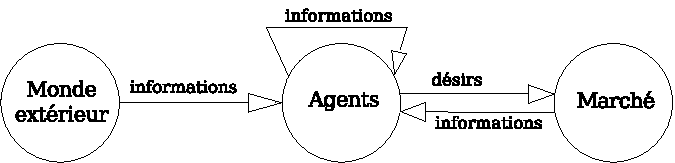
\includegraphics[width=.8\columnwidth]{marche.pdf}
  \end{center}

  \textbf{Implémentation}
  
  \begin{center}
    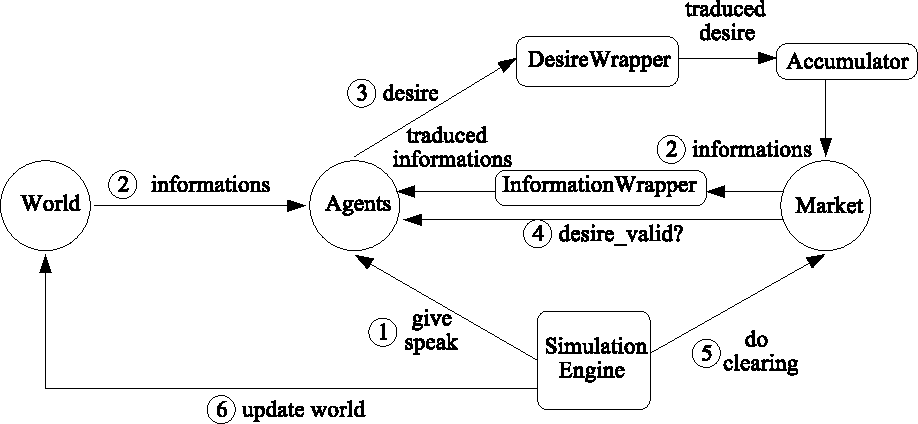
\includegraphics[width=.8\columnwidth]{modele.pdf}
  \end{center}
\end{frame}

%%%%%%%%%%%%%%%%%%%%%%%%%%%%%%%%%%%%%%%%%%%%%%%%%%%%%%%%%%%%%%%%%%%%%%%%%%%%%%

\begin{frame}
  \frametitle{Points importants}

  \textbf{Modèles agents}

  \begin{itemize}
  \item rôles
  \item interactions
  \item gestion du temps
% passage de parole entre agents
  \end{itemize}

  \vfill

  \textbf{Limites de l'informatique}

  \begin{itemize}
  \item calculs réels faux (souvent \textbf{très} faux)
  \item aléatoire inexistant (générateur pseudo aléatoire)
  \end{itemize}
\end{frame}

%%%%%%%%%%%%%%%%%%%%%%%%%%%%%%%%%%%%%%%%%%%%%%%%%%%%%%%%%%%%%%%%%%%%%%%%%%%%%%

\begin{frame}
  \frametitle{Choix des outils}
  
  \textbf{Développement ad-hoc}

  {\small\slshape L'informatique comme les mathématiques doit s'apprendre avant d'être utilisée}

  \vfill
  
  \textbf{Plateformes \emph{adaptées} existantes}

  {\small\slshape Netlogo, Repast, Atom, etc.}

  \vfill

  \textbf{Penser aux observations}

  {\small\slshape
    \begin{itemize}
    \item que doit-on observer~? comment~?
    \item outillage intégré, séparé
    \end{itemize}
  }
\end{frame}
  
%%%%%%%%%%%%%%%%%%%%%%%%%%%%%%%%%%%%%%%%%%%%%%%%%%%%%%%%%%%%%%%%%%%%%%%%%%%%%%

\begin{frame}
  \frametitle{Liens}

  \textbf{SMAC}{\hfill\footnotesize\url{http://www.lifl.fr/SMAC}}

  \vfill

  \begin{itemize}
  \item \textbf{IODA}\\
    Interaction-Oriented Design of Agents simulations

    {\null\hfill\footnotesize\url{http://www.lifl.fr/SMAC/projects/ioda}}

  \vfill

  \item \textbf{ATOM} ArTificial Open Market

    {\null\hfill\footnotesize\url{http://atom.univ-lille1.fr}}
  \end{itemize}

  \vfill

  \textbf{Publication du modèle}

  \vfill

  \emph{UML for ABM} par Hughes BERSINI
  
  {\null\hfill\footnotesize\url{http://jasss.soc.surrey.ac.uk/15/1/9.html}}
\end{frame}

%%%%%%%%%%%%%%%%%%%%%%%%%%%%%%%%%%%%%%%%%%%%%%%%%%%%%%%%%%%%%%%%%%%%%%%%%%%%%%

\begin{frame}
  \frametitle{Crédits}

  \small

  \begin{itemize}
  \item Cette présentation et son code source sont mises à disposition
    selon les termes de la
    \href{https://creativecommons.org/licenses/by-nc-sa/3.0/fr/legalcode}{Licence
      Creative Commons Attribution - Pas d’Utilisation Commerciale - Partage
      dans les Mêmes Conditions 3.0 France} \ccbyncsa.

    \vfill

  \item La présentation au format PDF est disponible à {\footnotesize\url{http://bruno.boulgour.com/talks/2013-10-11-mageco}}

    \vfill

  \item Le code source LaTeX de la présentation est disponible à {\footnotesize\url{https://github.com/b3/talks-20131011-mageco}}

    \vfill
  \item La dernière modification de ce document a eu lieu le 7~février~2014 à 23h38 %TS
  \end{itemize}
\end{frame}

\end{document}

% Local Variables:
% time-stamp-line-limit:-20
% time-stamp-start: "le "
% time-stamp-end: " %TS"
% time-stamp-format: "%:d~%:b~%:y à %:Hh%2M"
% time-stamp-active: t
% End:
